%!TEX root = ../dokumentation.tex
\chapter{ReactJS}
\label{ch:reactJS}

\section{Allgemein}

\subsection{Einführung in das Framework}\label{sec:rEinf}

ReactJS ist eine von Facebook entwickelte JavaScript Bibliothek zur Entwicklung von Benutzeroberflächen. Im Gegensatz zu Angular ist ReactJS ein reines View-Framework. Das Framework wird unter anderem bei Facebook, Instagram, Netflix, Airbnb und dem Content Management System Wordpress eingesetzt. Es bietet einige Vorteile bei der Entwicklung von Anwendungen mit großen Benutzeroberflächen mit Daten, die sich häufig verändern. 

Das Framework ist in JavaScript geschrieben und kann mit JavaScript oder einer in JavaScript übersetzbare Sprache wie TypeScript verwendet werden.\autocites[vgl.][1\psqq]{Gackenheimer.2015}[vgl.][3\psqq]{Zeigermann.2016}

\subsection{Vorbereitung der Entwicklungsumgebung}\label{sec:rEntw}
Für die Entwicklung einer React-Anwendung wird unter anderem \textit{NodeJS} (siehe \autoref{NodeJS}), ein Übersetzer (bspw. \textit{Babel} siehe \autoref{Babel}), ein Modul-Loader (bspw. \textit{Webpack} siehe \autoref{Webpack}) und die React-Bibliothek benötigt. Die React-Bibliothek bestehendes aus \textit{react} und \textit{react-dom} kann über den Paketmanager \textit{npm} installiert werden. \autocites[vgl.][92\psqq]{Stefanov.2017}[vgl.][8\psqq]{Zeigermann.2016}

Das Framework React kann nur zum Bilden von Benutzeroberflächen verwendet werden. Darüber hinaus bietet es keine weiteren Funktionen. Für die Entwicklung einer größeren Anwendung muss beispielsweise eine Router-Implementierung eingebunden und ein Architekturmodell definiert werden.
Sowohl \textcite{Zeigermann.2016} als auch \textcite{Stefanov.2017} empfehlen die Verwendung des Architekturmodells Flux und der Implementierung Redux. Flux beschreibt ein Anwendungsmodell, bei dem die Daten ausschließlich in eine Richtung fließen. \autocites[vgl.][8]{Zeigermann.2016}[vgl.][11]{Zeigermann.2016}[vgl.][167]{Stefanov.2017} 

\section{Architektur}
Zur Erklärung der Grundkonzepte wird das Hello Beispiel aus \autoref{BeschreibungHelloBsp} herangezogen.

\subsection{Das Wurzelelement}\label{sec:rWurz}

Eine React-Anwendung benötigt ein Wurzelelement auf einer HTML-Seite. Unter diesem HTML-Element rendert React die Benutzeroberfläche der React-Anwendung. Das Rendern bezeichnet dabei den Vorgang, der schlussendlich zum Einfügen von HTML-Elementen im DOM führt. Dieser Vorgang wird in \autoref{Rendern} näher betrachtet. 

Die Benutzeroberfläche einer React-Anwendung wird durch React-Elemente repräsentiert. Ein React-Element ist ein JavaScript-Objekt. Es ist unveränderbar und kann nur durch Erzeugen eines neuen Elements aktualisiert werden.

Das \autoref{lst:BeispielReactHtml} zeigt die HTML-Seite der Beispielanwendung. Die Benutzeroberfläche der Beispiel React-Anwendung aus \autoref{lst:BeispielReactRender} soll unter dem Element mit der ID \textit{app} gerendert werden. Dies erfolgt durch Aufruf der Methode \glqq ReactDOM.render() \grqq in \autoref{lst:BeispielReactRender}. Diese veranlasst React zum Rendern des im ersten Parameter definierten React-Elements in das im zweiten Parameter angegebenen Wurzelelements. Das React-Element wird unter Verwendung der Spracherweiterung JSX (siehe \autoref{sec:die-erweiterung-jsx}) definiert.

\begin{lstlisting}[caption=Beispiel React-Anwendung: HTML-Datei , label=lst:BeispielReactHtml, language=HTML]
<!DOCTYPE html>
<html>
	...
	<body>
		<div id="app"></div>
		<script src="src/app.js"></script>
	</body>
	...
</html>
\end{lstlisting}

In diesem Beispiel wird der Methode die Komponente App, die ein React-Element zurückliefert, übergeben. Auf die Komponenten wird in \autoref{sec:reactKomponenten} näher eingegangen. \autocites[vgl.][4\psqq, 26\psqq]{Zeigermann.2016}[vgl.][]{Facebook.2018}[vgl.][]{Facebook.2018c}[vgl.][2\psqq]{Stefanov.2017}


\begin{lstlisting}[caption=Beispiel React-Anwendung: Aufruf der Render-Methode, label=lst:BeispielReactRender, language=Java]
import "./styles.css";
import React from "react";
import ReactDom from "react-dom";
import Hello from "./hello";

class App extends React.Component {
	render() {	
		return (
			<ErrorBoundary>
				<Hello name="World" />
			</ErrorBoundary>
		);
	}
}

class ErrorBoundary extends React.Component {
	...	
}

ReactDom.render(<App />, document.getElementById("app"));
\end{lstlisting}


\subsection{Komponenten}\label{sec:reactKomponenten}

\comment{Events in React}

Komponenten sind das zentrale Element in ReactJS. Sie enthalten sowohl die Logik als auch die zugehörige Anzeige. Eine Komponente kann entweder als Klasse oder als Funktion (engl. functional components) implementiert werden. 

Eine Funktion, die eine React-Komponente implementiert, muss genau ein React-Element als Rückgabewert zurückgeben. Die Klasse muss von \textit{React.Component} erben und die Methode \textit{render()}, die ein React-Element zurückgibt, implementieren. Der Klassenname oder der Funktionsname entspricht dem Namen der Komponente.\autocite[vgl.][80\psqq]{Zeigermann.2016} Das \autoref{lst:BeispielReactHello} zeigt eine Komponente Hello, die als Komponentenklasse implementiert ist. 


\begin{lstlisting}[caption=Beispiel React-Anwendung: Die Komponente Hello, label=lst:BeispielReactHello, language=Java]
import "./styles.css";
import React from "react";
import ReactDom from "react-dom";

export default class Hello extends React.Component {
	constructor(props) {
		super(props);
		this.state = { name: this.props.name };
	}
	
	onChange(event) {
		this.setState({ name: event.target.value });
	}

	render() {
		return (<div>
			<h1>Hello {this.state.name}</h1>
			<input onChange={e => this.onChange(e)} />
		</div>);
	}
}
\end{lstlisting}

Durch Eigenschaften (engl. Properties) lässt sich das Aussehen und Verhalten einer Komponente von außen beeinflussen. Einer Komponente können Eigenschaften (engl. Properties) in Form eines Objektes übergeben werden. Das Propertie-Objekt kann von der Komponente nicht verändert werden. 

Bei Komponentenfunktionen wird das Objekt der Funktion und bei Komponentenklassen dem Konstruktor der Klasse übergeben. Nach der Weitergabe des Objekts an die Oberklasse React.Component stehen die Properties über die Instanzvariable \textit{props} zur Verfügung. \autocites[vgl.][24\psq,83-88]{Zeigermann.2016}[vgl.][12-17]{Stefanov.2017}

%Die von einer Komponente erwarteten Eigenschaften können über das Objekt \textit{propTypes} beschrieben werden. Das Objekt \textit{defaultProps} ermöglicht zudem das Bestimmen von Default-Werten für die Eigenschaften. Bei Komponentenfunktionen muss das Objekt als Eigenschaft der Funktion und bei Komponentenklassen als statisches Attribut an die Klasse gesetzt werden. Dies hat den Vorteil das React diese zur Laufzeit überprüfen und eine entsprechende Warnung ausgeben kann. Zudem kann der Entwickler auf einen Blick die von einer Komponenten erwarteten Eigenschaften erkennen. 

Die Komponentenklasse bietet gegenüber der Komponentenfunktion einige zusätzliche Funktionen. Eine  Komponente, die als Klasse implementiert wird, hat einen Zustand (engl. State). Dieser wird in der Instanzvariable \textit{state} gehalten und kann nur von der Komponente gelesen und verändert werden. Die Änderung des States sollte hauptsächlich über die Methode \textit{setState()} erfolgen. Diese Methode  erwartet ein Objekt mit KeyValue-Paaren oder eine Callback-Funktion. Durch den Aufruf der Methode wird der State mit dem bisherigen State zusammengeführt.\autocites[vgl.][24\psq,89-93]{Zeigermann.2016}[vgl.][17\psq]{Stefanov.2017} 

Die Komponente Hello in \autoref{lst:BeispielReactHello} verwendet einen über die Properties übergebenen Namen als initialen Wert für den im State gehaltenen Namen. Bei Änderungen im Inputfeld wird das Event OnChange ausgelöst, die Methode OnChange aufgerufen und der vom State gehaltene Namen über die Methode setState geändert. Der Aufruf der Methode führt zum erneuten Rendern der Anwendung. Der in der Überschrift angezeigte Name wird angepasst.

Eine Komponente hat einen gewissen Lebenszyklus. In diesen Zyklus kann bei Verwendung einer Komponentenklasse durch Überschreiben von Lebenszyklus-Methoden (engl. lifecycle-methods) eingegriffen werden. Die \autoref{fig:LifecyleComponent} zeigt die gebräuchlichsten Lebenszyklus-Methoden einer Komponente.\autocites[vgl.][96-100]{Zeigermann.2016}[vgl.][]{Facebook.2018b}

In einer Komponente können weitere Komponenten eingebunden werden. Eine Komponente wird dabei durch ihren Namen identifiziert. Das Einbinden erfolgt durch Verwendung der Komponente in der Ausgabe. Dieser können Attribute über die Properties mitgegeben werden.\autocites[vgl.][111\psqq]{Zeigermann.2016} In diesem Beispiel wird die Komponente Hello aus \autoref{lst:BeispielReactHello}  und die Komponente ErrorBoundary aus \autoref{lst:BeispielReactRender} in der Komponente App verwendet. 

%Beschreibung des Lebenszyklusses einer Komponente

\begin{figure}
	\centering
	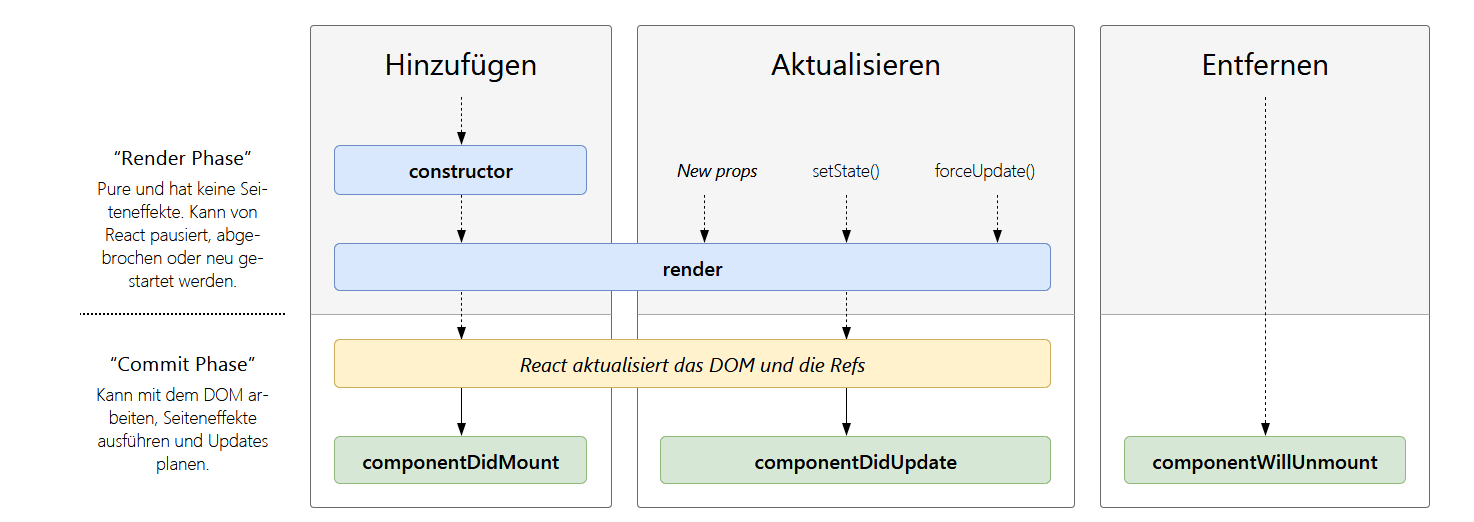
\includegraphics[width=\linewidth]{ReactLifecycle.png}
	\caption{Lebenszyklus einer  React-Komponente} 
	\quelle{\textcite{Maj.2018}}
	\label{fig:LifecyleComponent}
\end{figure}


\comment{abschließende Beschreibung des Bsp}

\subsection{Rendern von Komponenten}
\label{Rendern}
Eine Änderung an den Properties oder am State einer Komponente veranlasst React zum erneuten Rendern. Beim Rendern wird das von einer Komponente bereitgestellte React-Element allerdings nicht direkt in ein DOM-Element umgewandelt und in das native DOM eingesetzt. An stattdessen wird beim Aufruf der Render-Methode eine virtuelle Repräsentation des DOM-Baums generiert.

Anschließend vergleicht React den virtuellen DOM-Baum vor und nach der Änderung. Auf Grundlage der ermittelten Unterschiede generiert React eine minimale Anzahl an DOM-Operationen.  Diese Operationen werden dann auf den nativen DOM-Baum angewandt und stellen somit den gewünschten Zustand her. Das Rendern ist ein asynchroner Vorgang. Änderungen werden zum Teil zusammengefasst und nicht sofort angewandt.

React-Elemente sind einfache und leichtgewichtige JavaScript-Objekte. Daher können die Änderungen zwischen den zwei virtuellen DOM-Bäumen schnell ermittelt werden. Durch dieses Verfahren werden teure DOM-Manipulationen reduziert und damit die Performance der Web-Anwendung verbessert.\autocites[vgl.][23\psq,60\psq,90\psq]{Zeigermann.2016}[vgl.][53\psq]{Stefanov.2017}[vgl.][]{Facebook.2018}

\section{Verwendung}


